\documentclass[11pt]{beamer}

\mode<presentation>
\usetheme{Frankfurt}

\setbeamertemplate{caption}[numbered]

\usepackage[utf8]{inputenc}
\usepackage{amsmath}
\usepackage{amsfonts}
\usepackage{amssymb}
\usepackage{gensymb}
\usepackage{tikz}

\usetikzlibrary{arrows.meta}

\author{Alexey L. Cherezov}
\title{FRAPCON and RAST-K Coupling}
%\setbeamercovered{transparent} 
%\setbeamertemplate{navigation symbols}{} 
%\logo{} 
\institute{UNIST Core} 
%\date{} 
%\subject{} 


\tikzset{%
  >={Latex[width=2mm,length=2mm]},
  % Specifications for style of nodes:
            base/.style = {rectangle, rounded corners, draw=black,
                           minimum width=4cm, minimum height=1cm,
                           text centered, font=\sffamily},
  box0/.style = {base, minimum width=2.5cm, fill=white!30},
  box1/.style = {base, minimum width=2.5cm, fill=green!15},
  box2/.style = {base, minimum width=2.5cm, fill=orange!15},
  void/.style = {base, minimum width=2.5cm, fill=white!30, draw=white, align=left},
}


\begin{document}

\titlepage


\begin{frame}{Code structure}

\footnotesize


  \begin{columns}

  \column{0.25\textwidth}

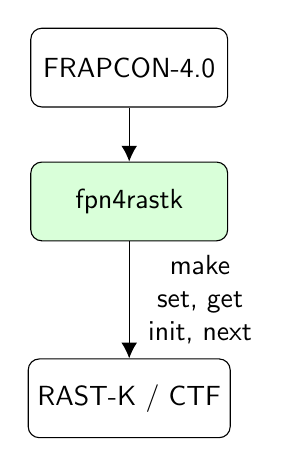
\begin{tikzpicture}[node distance=1.5cm, every node/.style={fill=white, font=\sffamily}, align=center]

  % Specification of nodes (position, etc.)
  \node (onFrapcon)    [box0]                                  {FRAPCON-4.0};
  \node (onFpn4rastk)  [box1, below of=onFrapcon, yshift=-0.2cm] {fpn4rastk};  
  \node (onRastk)      [box0, below of=onFpn4rastk, yshift=-1.0cm] {RAST-K / CTF};  
  
  % Specification of lines between nodes specified above
  % with aditional nodes for description 
  \draw[->]      (onFrapcon) --                                (onFpn4rastk);
  \draw[->]      (onFpn4rastk) -- node [xshift=0.9cm] {make \\ set, get \\ init, next}                      (onRastk);  
  \end{tikzpicture}
  
  \column{0.75\textwidth}

  \begin{block}{}
    \texttt{{\color{magenta}PROGRAM}}\\
    \texttt{{\color{magenta}USE} fpn4rastk, {\color{magenta}ONLY} : MAKE, INIT, NEXT, SET, GET}
    \begin{itemize}
    \item \texttt{{\color{magenta}CALL} MAKE(<arguments>)}
    \item \texttt{{\color{magenta}CALL} SET({\color{orange}"name"}, variable)}    
    \item \texttt{{\color{magenta}CALL} INIT()}    
    \end{itemize}
    \texttt{{\color{magenta}DO} i = 1, N}        
    \begin{itemize}
    \item \texttt{{\color{magenta}CALL} SET({\color{orange}"name"}, variable)}
    \item \texttt{{\color{magenta}CALL} NEXT(dtime)}        
    \item \texttt{{\color{magenta}CALL} GET({\color{orange}"name"}, variable)}
    \end{itemize}
    \texttt{{\color{magenta}ENDDO}} \\
    \texttt{{\color{magenta}END PROGRAM} }        
  \end{block}

  \end{columns}

\end{frame}

\begin{frame}{Capability of the fpn4rastk module}
  \footnotesize

  \begin{block}{Time integration:}
  \begin{itemize}
    \item ...
  \end{itemize}
  \end{block}

  \begin{block}{Switched off models:}
  \begin{itemize}
    \item Decay model ANS-5.1 (2005)
    \item Fission gas response model ANS-5.4 (1952)
  \end{itemize}
  \end{block}

\end{frame}


\begin{frame}{Running calculations: Initialization}
  
  \footnotesize

  \begin{block}{Initialization: \texttt{make(m,n,dx,rf,rg,rc,pitch,den,enrch)}}
    \begin{itemize}
    \item \texttt{m, n} : number of radial and axial segments
    \item \texttt{dx} : axial node thickness, cm
    \item \texttt{rfuel, rgap, rclad} : radius of fuel, gap and cladding, cm
    \item \texttt{pitch} : fuel rod pitch, cm
    \item \texttt{den} : as-fabricated apparent fuel density, $\%$
    \item \texttt{enrch} : initial fuel enrichment, $\%$
    \end{itemize}
  \end{block}

\end{frame}



\begin{frame}{Running calculations: Settings of parameters}
  
  \footnotesize

  \begin{block}{Set variables : \texttt{set(key, value)}}
    \begin{itemize}
    \item \texttt{key} : name of the variable
    \item \texttt{value} : value of the variable    
    \end{itemize}
  \end{block}

  \begin{block}{List of the available parameters}
    \begin{itemize}
    \item linear power distribution, $\frac{W}{cm}$
    \item coolant temperature distribution, $\degree C$
    \item coolant pressure distribution, $MPa$
    \item coolant mass flux, $\frac{kg}{s \cdot m^2}$
    \end{itemize}
  \end{block}

\end{frame}



\begin{frame}{Running calculations: Time step}
  
  \footnotesize

  \begin{block}{Very first time step: \texttt{init()}}
  The first time step is needed in order to stabilize the time-integration scheme
  \end{block}

  \begin{block}{Next time step: \texttt{next(dtime)}}
    \begin{itemize}
    \item \texttt{dtime} : time step, $day$
    \end{itemize}
  \end{block}

\end{frame}


\begin{frame}{Running Calculations: Output Data}
  
  \footnotesize

  \begin{block}{Get variables: \texttt{get(key, value)}}
    \begin{itemize}
    \item \texttt{key} : name of the variable
    \item \texttt{value} : value of the variable    
    \end{itemize}
  \end{block}
  
  \begin{columns}
  \column{0.49\textwidth}
  \begin{block}{List of the available parameters}
    \begin{itemize}
    \item axial fuel temperature, $\degree C$
    \item bulk coolant temperature, $\degree C$
    \item gap conductance, $\frac{W}{m^2 \cdot K}$
    \item thermal gap thickness, $\mu m$
    \item mechanical gap thickness, $\mu m$
    \end{itemize}
  \end{block}

  \column{0.49\textwidth}  
  \begin{block}{}
    \begin{itemize}
    \item gap pressure, $MPa$
    \item cladding hoop strain, $\%$
    \item cladding hoop stress, $MPa$
    \item cladding axial stress, $MPa$
    \item cladding radial stress, $MPa$
    \item cladding radial stress, $MPa$
    \item axial mesh, $cm$
    \end{itemize}
  \end{block}

  \end{columns}

\end{frame}


\begin{frame}{Test Example}
  
  \footnotesize

  \begin{block}{Fuel rod}
    \begin{itemize}
    \item Uranium fuel rod with the initial enrichment $x=3.42\%$    
    \item Fuel pellet diameter $d=8.26 mm$, length $h=9.8298 mm$
    \item Fuel stack height $H=3.8333 m$, plenum length $L=16.1 cm$
    \end{itemize}
  \end{block}

  \begin{block}{Initial conditions}
    \begin{itemize}
    \item Average linear heat rating is 14.6 $kW/m$
    \item Coolant inlet temperature is 569 $K$
    \item Coolant mass flux is 3857 $\frac{kg}{s \cdot m^2}$
    \end{itemize}
  \end{block}

  \begin{block}{Transient simulation}
    \begin{itemize}
    \item Transient during 40 days with the time step 5 days
    \item Input parameters are changed: $C(t) = C_0 Sin(\pi t/T)$, where $T=20$ days
    \end{itemize}
  \end{block}

\end{frame}



\begin{frame}{Input parameters}
  \footnotesize 
  
  \begin{columns}[t]

  \column{.49\textwidth}

  \begin{figure}[h]
    \includegraphics[width=1.\textwidth]{figs/axial_fuel_temperature}
    \caption{Axial fuel temperature}
    \label{fig:tfuel}
  \end{figure}  

  \column{.49\textwidth}

  \begin{figure}[h]
    \includegraphics[width=1.\textwidth]{figs/bulk_coolant_temperature}    
    \caption{Bulk coolant temperature}
    \label{fig:tcool}
  \end{figure}  
  
  \end{columns}

\end{frame}



\begin{frame}{Output parameters (1)}
  \footnotesize 
  
  \begin{columns}[t]

  \column{.49\textwidth}

  \begin{figure}[h]
    \includegraphics[width=1.\textwidth]{figs/gap_conductance}
    \caption{Gap conductance}
    \label{fig:conduct}    
  \end{figure}  

  \column{.49\textwidth}

  \begin{figure}[h]
    \includegraphics[width=1.\textwidth]{figs/oxide_thickness}    
    \caption{Oxide thickness}
    \label{fig:oxide}
  \end{figure}  
  
  \end{columns}

\end{frame}


\begin{frame}{Output parameters (2)}
  \footnotesize 
  
  \begin{columns}[t]

  \column{.49\textwidth}

  \begin{figure}[h]
    \includegraphics[width=1.\textwidth]{figs/mechanical_gap_thickness}
    \caption{Mechanical gap thickness}
  \end{figure}  

  \column{.49\textwidth}

  \begin{figure}[h]
    \includegraphics[width=1.\textwidth]{figs/gap_pressure}    
    \caption{Gap pressure}
  \end{figure}  
  
  \end{columns}

\end{frame}

\begin{frame}{Output parameters (3)}
  \footnotesize 
  
  \begin{columns}[t]

  \column{.49\textwidth}

  \begin{figure}[h]
    \includegraphics[width=1.\textwidth]{figs/cladding_hoop_strain}
    \caption{Cladding hoop strain}
  \end{figure}  

  \column{.49\textwidth}

  \begin{figure}[h]
    \includegraphics[width=1.\textwidth]{figs/cladding_axial_stress}    
    \caption{Cladding axial stress}
  \end{figure}  
  
  \end{columns}

\end{frame}

\end{document}

